% Chapter 5: Outlook
% Contains:
%   The non-uniform case
%   The multiplicative coalescence
%   Open questions?

\chapter{Outlook} \label{C: outlook}

This chapter will give a brief overview of the results obtained in the remainder of Aldous paper,
and introduce the questions left open by the end as well as further research into these.

\section{The non-uniform case}

\begin{figure}[H]
	\centering
	\subfloat[A graph component]
	{\begin{tikzpicture}[level distance = 11mm, scale = 1]
\tikzstyle{level 1}=[sibling distance=8mm]
\tikzstyle{level 2}=[sibling distance=8mm]
\tikzstyle{level 3}=[sibling distance=8mm]


% VERTICES
\node [plain, minimum size = 1.46em, inner sep = 0.5] (1) {1} [grow=up]
	child { node [plain, minimum size = 1.55em, inner sep = 0.5] (3) {3}
		child { node [plain, minimum size = 1.15em, inner sep = 0.5] (5) {5}
		}
		child { node [plain, minimum size = 1.52em, inner sep = 0.5] (4) {4}
		}
	}
	child { node [plain, minimum size = 1.38em, inner sep = 0.5] (2) {2}
}
;
\node [plain, minimum size = 1.43em, inner sep = 0.5] [right=1cm of 1] (6) {6}
;
\node [plain, minimum size = 1.15em, inner sep = 0.5] [right=1cm of 6] (7) {7} [grow=up]
	child { node [plain, minimum size = 1.41em, inner sep = 0.5] (8) {8}
}
;
%1.42 1.26 1.60 1.54 1.00 1.37 1.00 1.32
%1.46 1.38 1.55 1.52 1.23 1.43 1.23 1.41

% WEIGHTS LABELS
\node[below right=-0.1cm of 1] {0.8};
\node[below left=-0.1cm of 2] {0.5};
\node[below right=-0.1cm of 3] {1.3};
\node[below left=-0.1cm of 4] {1.1};
\node[below right=-0.1cm of 5] {0.2};
\node[below right=-0.1cm of 6] {0.7};
\node[below right=-0.1cm of 7] {0.2};
\node[below right=-0.1cm of 8] {0.6};





\end{tikzpicture}
}\\
	
	\centering
	\subfloat[The continuous-time breadth-first walk]
	{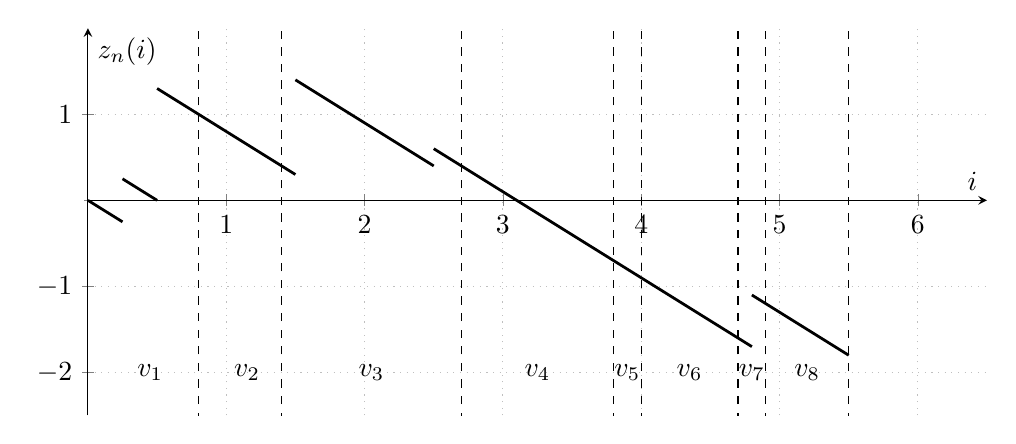
\begin{tikzpicture}

\begin{axis}[
axis x line=bottom,
axis y line=left,
grid = minor,
minor grid style={dotted},
xmin=0,
axis lines = middle,
xmax=6.5,
ymax = 2,
ymin  = -2.5,
xlabel={$i$},
%x label style = {at={(axis description cs:1.04,0.785)},anchor=east},
ylabel={$z_n(i)$},
%y label style = {at={(axis description cs:0,1.11)},anchor=north},
xtick={1,...,6},
minor xtick = {1,...,6},
ytick={-2,...,1},
minor ytick={-2,...,1},
width = 13cm,
height = 6.5cm
]


% BF WALK LINE
\addplot [line width=1.0pt]coordinates{(0,0) (0.25,-0.25)}; 
% JUMP 0.5
\addplot [line width=1.0pt]coordinates{(0.25,0.25) (0.5,0)}; 
% JUMP 1.3
\addplot [line width=1.0pt]coordinates{(0.5,1.3) (0.9,0.9)};

\addplot [line width=1.0pt]coordinates{(0.9,0.9) (1.5,0.3)}; 
% JUMP 1.1
\addplot [line width=1.0pt]coordinates{(1.5, 1.4) (2.5, 0.4)};
% JUMP 0.2
\addplot [line width=1.0pt]coordinates{(2.5, 0.6) (4.8,-1.7)};
% JUMP 0.6
\addplot [line width=1.0pt]coordinates{(4.8,-1.1) (5.5,-1.8)};

% VERTEX BORDERS
\addplot [dashed] coordinates {(0.8, -7) (0.8, 2)};
\addplot [dashed] coordinates {(1.4, -7) (1.4, 2)};
\addplot [dashed] coordinates {(2.7, -7) (2.7, 2)};
\addplot [dashed] coordinates {(3.8, -7) (3.8, 2)};
\addplot [dashed] coordinates {(4.0, -7) (4.0, 2)};
\addplot [dashed] coordinates {(4.7, -7) (4.7, 2)};
\addplot [dashed] coordinates {(4.9, -7) (4.9, 2)};
\addplot [dashed] coordinates {(5.5, -7) (5.5, 2)};

% VERETX LABELS
\node at (axis cs:0.45,-2) {$v_1$};
\node at (axis cs:1.15,-2) {$v_2$};
\node at (axis cs:2.05,-2) {$v_3$};
\node at (axis cs:3.25,-2) {$v_4$};
\node at (axis cs:3.9,-2) {$v_5$};
\node at (axis cs:4.35,-2) {$v_6$};
\node at (axis cs:4.8,-2) {$v_7$};
\node at (axis cs:5.2,-2) {$v_8$};

\end{axis}

\end{tikzpicture} }
	
	\caption{Continuous breadth-first walk on a single component}
	\label{F: inh bf-walk cont}
\end{figure} 


\section{The multiplicative coalescence}



\section{Further results}